\documentclass[bibliography=totoc]{scrartcl}
\usepackage[ngerman, english]{babel}
\usepackage{rwukoma}
\usepackage[pdfusetitle]{hyperref}
\usepackage{lipsum,caption}
\usepackage{acronym}
\usepackage{algorithm, algpseudocode}
\usepackage{graphicx}
\usepackage{subcaption}
\usepackage{listings}
\usepackage{float}
\usepackage{todonotes}
\usepackage{amsmath}
\usepackage{comment}

\setlength{\belowcaptionskip}{5pt}

\title{Comparison of different path planning algorithms}
\author{Manuel Gnannt - 34946, IN \\ Florian Betz - 35653, IN}
\date{13.03.2023}%\today}
\begin{document}
\maketitle
\tableofcontents

\clearpage
\section{Abstract}
In path planning, discovering good trajectories often requires a high-dimensional model and the evaluation of many samples. Recently, Wang et al. proposed an algorithm called \textbf{La}tent Space \ac{LaP3} claiming it outperforms existing path planning methods in 2D navigation tasks with respect to sample efficiency. In this paper, we compare the newly published \ac{LaP3} to other path-planning algorithms in several 2D environments.
\todo[inline]{extend descriptions with all information}
%\todo[inline]{problems, why, solutions, results}

\section{Introduction}
In path planning, the goal is to find the most rewarding trajectory in a given search space. 

A common problem faced by approaches like \ac{CMA-ES} \cite{CMA-ES} is being trapped at local optima. 
Another is the exploration-exploitation tradeoff. 
Approaches like \ac{VOOT} \cite{VOOT} try to tackle both the local optimum problem and the exploration-exploitation tradeoff by partitioning the search space.
This partitioning however is done independently from the reward function, making it less efficient.

For a more efficient search space partitioning, Wang et al. proposed \ac{LaP3} an extension of \ac{La-MCTS} \cite{La-MCTS} where the search space is  partitioned into high- and low-reward regions thus splitting is done based on the reward function.
%The main difference between \ac{LaP3} and \ac{La-MCTS} is a different calculation of the node values and additional sampling via \ac{CMA-ES} instead of Bayesian Optimization.

This paper explores the topic of path planning, with a focus on three specific algorithms A*, \ac{La-MCTS}, and \ac{LaP3}. 

\section{Path Planning Algorithms}
\label{path_planning_algorithm}
In this paper, we decided to use three different search algorithm A*, \ac{La-MCTS} and \ac{LaP3}.

\subsection{A*}
%\todo[inline]{image? Zitat, Florian}
%\todo[inline]{Seite + Zeilen zu jedem Zitat (Text und image), Florian}

The A* algorithm, first introduced by Peter Hart and other researchers at the Stanford Research Institute in 1968, is a widely used method for pathfinding and graph traversal. \cite{4082128} It builds on Dijkstra's algorithm by incorporating heuristic functions and predicted costs, making it the most efficient direct search method for finding the shortest paths in a static road network and a popular heuristic for various other problems.\cite{ProbabilisticApproachCollaborativeMultiRobotLocalization}

The key component of the algorithm is the design of the valuation function, $f(n) = g(n) + h(n)$, where $g(n)$ is the actual cost from the initial node to node n, $h(n)$ is the estimated cost from node n to the target node, and $f(n)$ is the estimated cost from the initial node via node n to the target node. The A* algorithm can reach a time complexity of $O(n)$.

\textbf{Step 1:} Add the starting node to the priority queue.
\newline
\textbf{Step 2:} Select the node with the smallest F-value from the current priority queue and make it the current node. Use the Euclidean Distance Heuristics from figure \ref{fig:EuclideanDistanceHeuristics}
\newline
\textbf{Step 3:} Mark it as visited and process its adjacent nodes.
\newline
\textbf{Step 4:} If the neighboring node has not been visited, add it to the queue, set the current node as its parent, and record its F, H, and G values. 
If the neighboring node has already been visited, check if the current node has a shorter path by comparing G values. See in figure \ref{fig:astar_path}.
If the current node has a smaller G value, update the parent node and G, H values of that node.
\newline
\textbf{Step 5:} Repeat steps 2 to 4 until the target node is marked or the priority queue is empty.
\newline
\textbf{Step 6:} When the path is found, trace back from the endpoint to the start node using the parent node.



\begin{figure}[H]
	\centering
	\begin{subfigure}[b]{0.3\linewidth}
		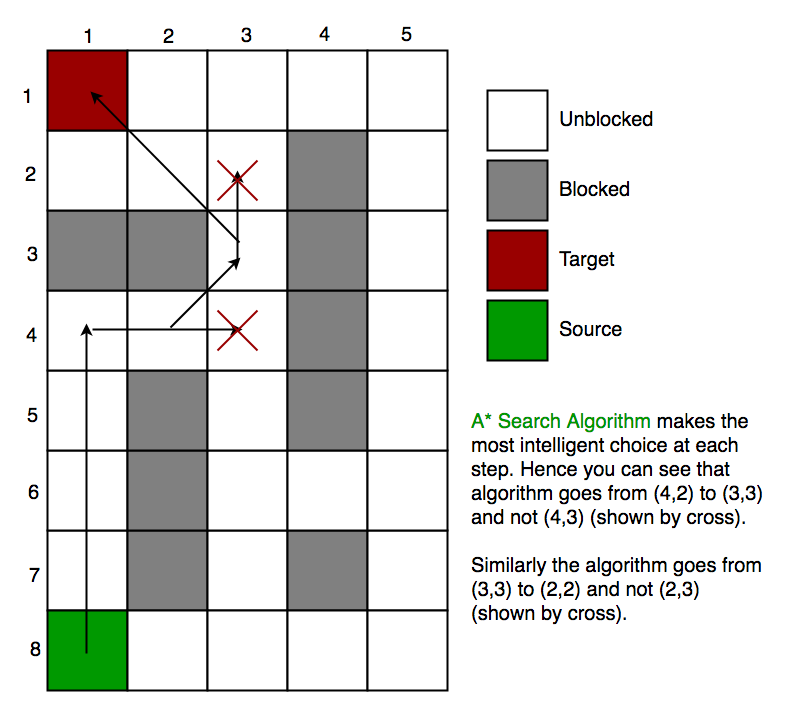
\includegraphics[width=\linewidth]{img/a_-search-algorithm.png}
        \caption{Astar path}
        \label{fig:astar_path}
        	
    \end{subfigure}
	\hspace{0.02\textwidth}
	\begin{subfigure}[b]{0.3\linewidth}
		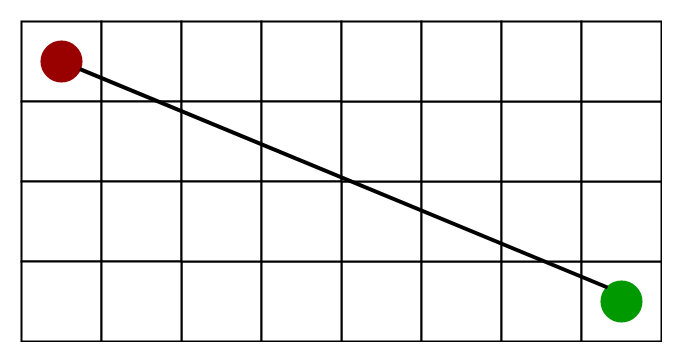
\includegraphics[width=\linewidth]{img/a_-search-algorithm-euclidian_distance.png}
		\caption{Euclidean Distance Heuristics}
        \label{fig:EuclideanDistanceHeuristics}
	\end{subfigure}
 	\caption{Astar \cite{Pic:astar}}
	\label{fig:astar}
\end{figure}

\newpage
\subsection{La-MCTS}
The basic idea of a \ac{La-MCTS} is to recursively split the search space with every region representing a node in a Monte-carlo tree.\cite{La-MCTS}
As shown in figure \ref{fig:laMCTS_sampling_splitting}, this is done by taking some samples from the search space and splitting it into a high- and a low-reward section using K-means (k=2). 
An \ac{SVM} then learns this boundary and the two sections can be represented as nodes in a monte carlo tree.
In our example, the high-reward section is represented by the left node and the low-reward section by the right node.


\begin{figure}[H]
	\centering
	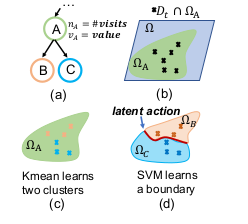
\includegraphics[width = {0.35\textwidth}]{img/lamcts_1.png}
	\caption{\ac{La-MCTS} sampling and splitting \cite{La-MCTS}[p.3]}
	\label{fig:laMCTS_sampling_splitting}
\end{figure}
As shown in in figure \ref{fig:laMCTS_workflow}, this process is now repeated by selecting a node until a leaf node is reached, taking samples along the corresponding section and splitting it again. 
This results in a tree structure with the leftmost node representing the section with the highest reward. 

\begin{figure}[H]
	\centering
	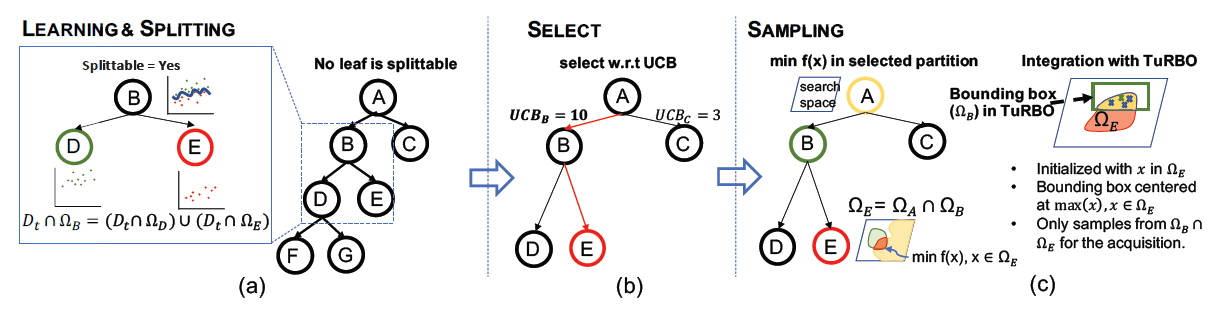
\includegraphics[width = {\textwidth}]{img/lamcts_workflow.png}
	\caption{Steps of \ac{MCTS} \cite{La-MCTS}[p.4]}
	\label{fig:laMCTS_workflow}
\end{figure}

\subsection{LaP3}
%https://www.youtube.com/watch?v=-4Lzk_s_Dzw
\ac{LaP3} works similar to \ac{La-MCTS}. The main difference is that after each sampling step, the whole tree is updated and not only a single leaf. Other differences are the method of determining the goodness of a node (\ac{LaP3} uses the maximum, where \ac{La-MCTS} uses the mean) and the sampling method (\ac{LaP3} uses \ac{CMA-ES} where \ac{La-MCTS} uses \ac{BO}).

\section{Methodology}
We ran \ac{LaP3}, \ac{La-MCTS} and an A* on two different environments with both environments containing local optima. For each environment, the experiment was run on a 12x12, a 24x24 and a 36x36 grid. As the goal is finding a sample efficient trajectory the number of samples was used as a metric in relation to the reward. The reward was calculated by the inverse of the euclidian distance to the target. It can be described by following formula. 

%\todo[inline]{formelzeichen beschreiben}

\begin{equation}
\left\{
\begin{array}{lll}
 r(\vec{x})=\frac{10}{\sqrt{\Delta x_1 ^2+\Delta x_2 ^2}}\quad \Delta x_1 + \Delta x_2 \neq 0\\
r(\vec{x})=15\quad \Delta x_1 + \Delta x_2 =0\\
\end{array}
\right.
\end{equation}

\begin{figure}[H]
	\centering
	\begin{subfigure}[b]{0.3\linewidth}
		\includegraphics[width=\linewidth]{img/Maze_s3.png}
        \caption{Maze S3 environemt}	
    \end{subfigure}
	\hspace{0.02\textwidth}
	\begin{subfigure}[b]{0.3\linewidth}
		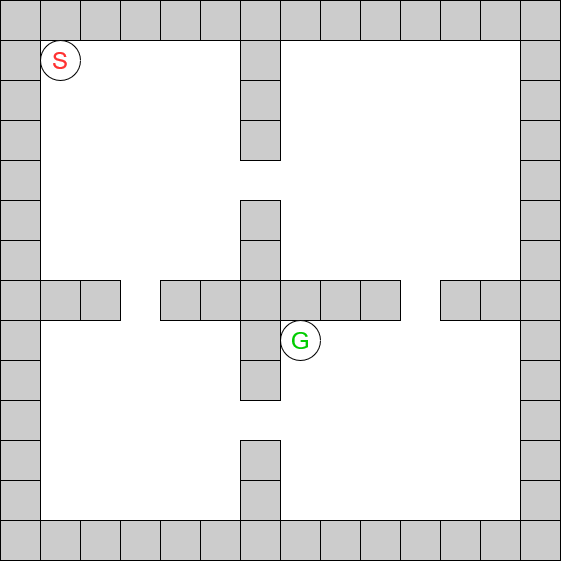
\includegraphics[width=\linewidth]{img/Four_Rooms.png}
		\caption{Four Rooms}
	\end{subfigure}
 	\caption{different environments}
	\label{fig:differentenvironments}
\end{figure}

\subsection{Search Efficiency}
The goal in path planning is to find the most rewarding trajectory in the search space.
As the optimum can eventually be found by random sampling if the number of samples is high enough, an efficient algorithm is preferred.
The search efficiency of an algorithm can therefore be described by the number of samples and the achieved reward.
As this metric is used widely when comparing different search algorithms, \cite{La-MCTS}, \cite{LaNAS}, \cite{VOOT}, we also used it for comparison.

\todo[inline]{LaNas wird als Acronym nicht verwendet}


\section{Evaluation}

%1. LaP3 Algorithmus wurde entwickelt, der die Pfade schneller berechnet
%2. LAP3 performt besser als der MCTS und A*
%3. Anhand gleicher Anzahl an samples ist der reward beim LAP3 immer besser
%4. verschiedene Metriken wurden verwenden space complexity, world environment
%5. Was sind unsere Ergebnisse, Performt LAP3 tatsächlich immer besser?
%6. Was kann in Zukunft noch nageschaut werden?

With the evaulation criteria and the different environment, the search algorithms are examined to see if the \ac{LaP3} performs better from several points of view.
Figure \ref{fig:SampleRewardMazeDifferentSpaceComplexity} shows the number of samples drawn and the associated reward in different environments with different complexities.
The environment is the maze s3 with complexity size 12x12, 24x24 and 36x36
The A* always delivers the same results, but \ac{La-MCTS} and \ac{LaP3} deliver different results on hundred runs and 
That is why the mean value and the lower and upper bound of the 95\% confidence interval are displayed in the graphs.
It can be seen that the \ac{LaP3} gets a larger reward than the \ac{La-MCTS} and A* with the same number of samples.
Although the \ac{LaP3} has a high variance, the reward increases consistently with increasing samples.
However, the \ac{LaP3} algorithm has a very large scattering of the delivered results.
For the \ac{La-MCTS}, an increase in variance does not occur until a sample size of 42 in a 12x12 environment and a sample size of 55 in a 24x24 and 36x36 environment.
The reward from the A* fluctuates continuously, but the reward does not increase as the number of samples increases.

\begin{figure}[H]
	\centering
	\begin{subfigure}[b]{0.3\linewidth}
		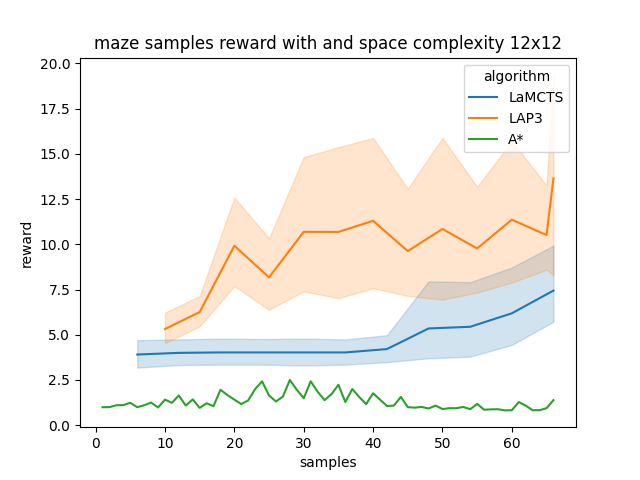
\includegraphics[width=\linewidth]{img/maze_samples__reward_b_8_LAP3_MCTS_AStar_interrupted_12.png}
        \caption{space complexity 12x12}	
    \end{subfigure}
	%\hspace{0.02\textwidth}
	\begin{subfigure}[b]{0.3\linewidth}
		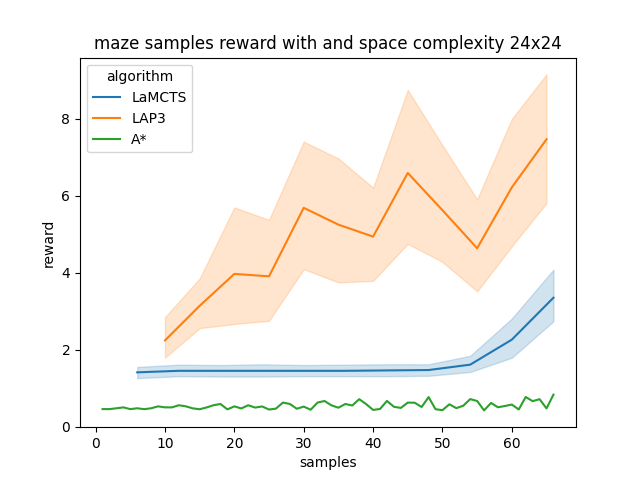
\includegraphics[width=\linewidth]{img/maze_samples__reward_b_8_LAP3_MCTS_AStar_interrupted_24.png}
		\caption{space complexity 24x24}
	\end{subfigure}
	%\hspace{0.02\textwidth}
	\begin{subfigure}[b]{0.3\linewidth}
		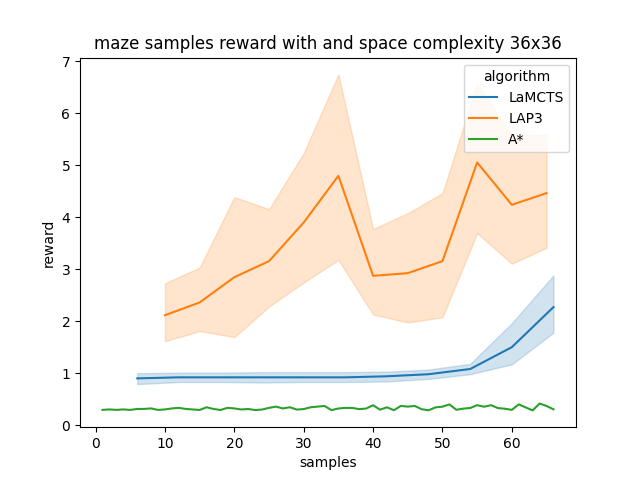
\includegraphics[width=\linewidth]{img/maze_samples__reward_b_8_LAP3_MCTS_AStar_interrupted_36.png}
        \caption{space complexity 36x36}
	\end{subfigure}
	\caption{ratio of samples and reward in Maze s3 environment with different space complexity}
	\label{fig:SampleRewardMazeDifferentSpaceComplexity}
\end{figure}

Figure \ref{fig:SampleRewardFourRoomsDifferentSpaceComplexity} shows the ratio of samples drawn and the associated reward in the four rooms environment with complexity size 12x12, 24x24 and 36x36.
As in the maze s3 environment, the A* generates a low reward with a low number of samples. 
Only in the 12x12 environent with a sample number of 40 does the reward increase and achieve a similar reward to the \ac{La-MCTS}.
With greater space complexity, the reward remains constantly low.
The \ac{La-MCTS} corresponds to a growing exponential function with constant mean.
The \ac{LaP3} on the other hand has a strong growth of the rewards at the beginning. With increasing sample number, however, the growth is reduced. However, the reward of \ac{LaP3} is larger than that of \ac{La-MCTS} and A* at each sample number.

\begin{figure}[H]
	\centering
	\begin{subfigure}[b]{0.3\linewidth}
		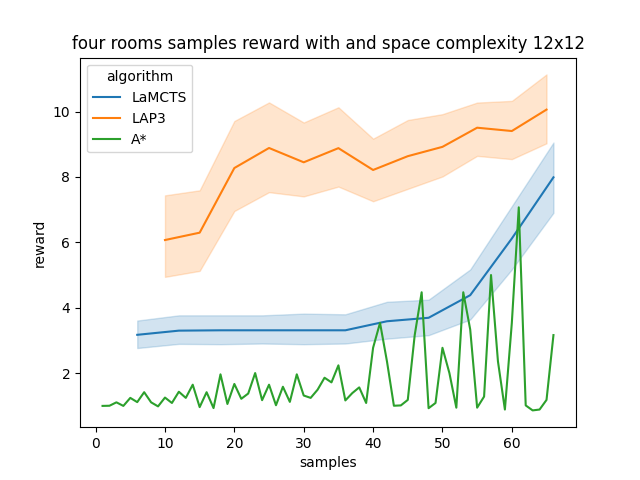
\includegraphics[width=\linewidth]{img/four_rooms_samples__reward_b_8_LAP3_MCTS_AStar_interrupted_12.png}
        \caption{space complexity 12x12}	
    \end{subfigure}
	\hspace{0.02\textwidth}
	\begin{subfigure}[b]{0.3\linewidth}
		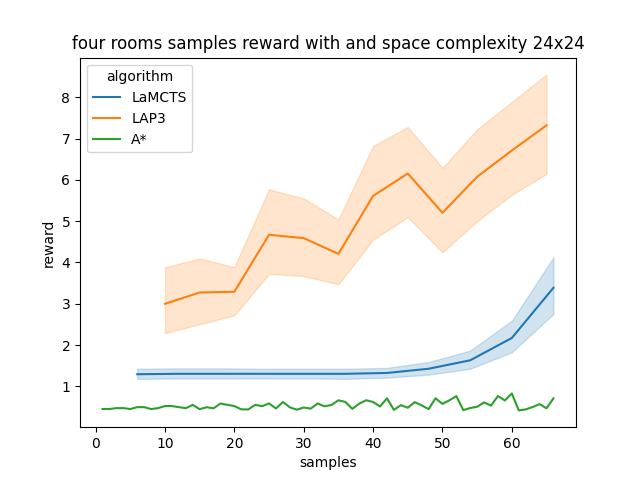
\includegraphics[width=\linewidth]{img/four_rooms_samples__reward_b_8_LAP3_MCTS_AStar_interrupted_24.png}
		\caption{space complexity 24x24}
	\end{subfigure}
	\hspace{0.02\textwidth}
	\begin{subfigure}[b]{0.3\linewidth}
		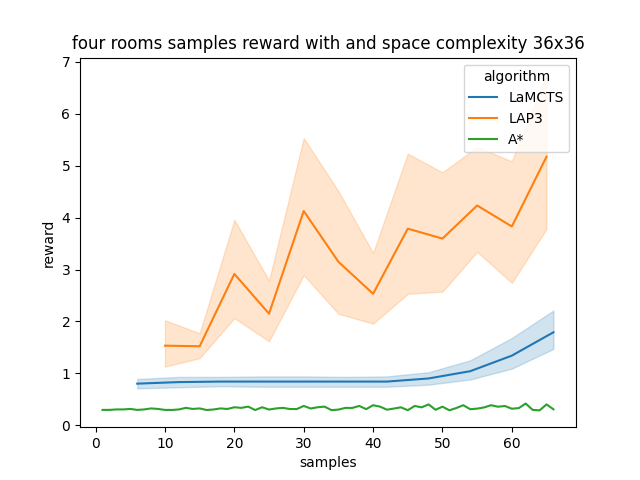
\includegraphics[width=\linewidth]{img/four_rooms_samples__reward_b_8_LAP3_MCTS_AStar_interrupted_36.png}
        \caption{space complexity 36x36}
	\end{subfigure}
	\caption{ratio of samples and reward in four rooms environment with different space complexity}
	\label{fig:SampleRewardFourRoomsDifferentSpaceComplexity}
\end{figure}

What is striking in both environments is that the \ac{La-MCTS} has a constant reward function. 
In the beginning, the reward is constant and increases exponentially after 40 samples.
The \ac{LaP3} exhibits significant variation in its reward data, although the specific mean values provided by the \ac{LaP3} are displayed in table \ref{tab:mean_std_diff_sizes}. 
As we can see in figure \ref{fig:maze_complexity_reward_lap3_lamcts_astar}, the complexity of the environment increases, the reward diminishes rapidly.

\begin{figure}[H]
	\centering
	\begin{subfigure}[b]{0.55\linewidth}
    	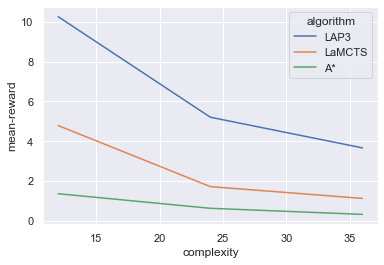
\includegraphics[width = {\textwidth}]{img/maze_complexity_reward_lap3_lamcts_astar.png}
    	\caption{maze s3 space complexity and mean reward $\overline{x}$}
    	\label{fig:maze_complexity_reward_lap3_lamcts_astar}	
    \end{subfigure}
	%\hspace{0.02\textwidth}
    \begin{subfigure}[b]{0.4\linewidth}
        \begin{tabular}{|c|c|c|c|c|}
        \hline
        & {12x12} & {24x24} & {36x36} \\ \hline
        Samples & $\overline{x}$ & $\overline{x}$ &  $\overline{x}$ \\ \hline
        20 &  9.9208     & 3.9697  & 2.8462 \\ \hline
        25 &  8.1711     & 3.9062  & 3.1538 \\ \hline
        30 &  7.4318     & 5.6875  & 3.8974 \\ \hline
        35 & 10.6842     & 5.2500  & 4.7949 \\ \hline
        40 & 11.3000     & 4.9394  & 2.8718 \\ \hline
        45 &  9.6250     & 6.5938  & 2.9231 \\ \hline
        50 & 10.8485     & 5.6250  & 3.1538 \\ \hline
        55 &  9.7692     & 4.6364  & 5.0513 \\ \hline
        60 & 11.3611     & 4.6364  & 4.2368 \\ \hline \hline
           & 10.2632     & 5.2030  & 3.6588 \\ \hline
        \end{tabular}
        \caption{mean and 95\% confidence interval of \ac{LaP3}}
        \label{tab:mean_std_diff_sizes}
    \end{subfigure}
    \caption{first 60 samples drawn in maze s3 environment with different complexity}
    %\label{fig:mean_complexity_reward}
\end{figure}

\todo[inline]{Aussage beantwortet, \ac{LaP3} performt immer besser}
\todo[inline]{Schaubild 7 beschreiben}
\todo[inline]{\ac{LaP3} beschreiben, dass man in ein locales minumu leicht reinkommt}

\section{Conclusions and Further Discussion}
Different sampling methods

\todo[inline]{What could be explorer in the future,Manuel}

\todo[inline]{functions evals?, Manuel}
\todo[inline]{sample drawing in sequential action space (horiyon tto draw samples from, not whole search space), Manuel}

\clearpage


\section*{Acronyms} 
\addcontentsline{toc}{section}{Acronyms}

\begin{acronym}[....]
    \acro{LaP3}{Latent Space Partitions for Path Planning}
    \acro{MCTS}{Monte Carlo Tree Search}
    \acro{La-MCTS}{Latent Action Monte Carlo Tree Search}
    %\acro{LaNas}{Latent Space Neural Architecture Search}
    \acro{CMA-ES}{Covariance matrix adaptation evolution strategy}
    \acro{BO}{Bayesian Optimization}
    \acro{VOOT}{Voronoi Optimistic Optimization Tree}
    \acro{SVM}{Support vector machine}
\end{acronym}

\bibliographystyle{alpha}
\bibliography{literature}
\end{document}
